\documentclass[journal]{IEEEtran}
\usepackage{amsmath,amssymb,amsfonts}
\usepackage{tabularx}
\usepackage[utf8]{inputenc} % allow utf-8 input
\usepackage[T1]{fontenc}    % use 8-bit T1 fonts
\usepackage{url}            % simple URL typesetting
\usepackage{booktabs}       % professional-quality tables
\usepackage{amsfonts}       % blackboard math symbols
\usepackage{nicefrac}       % compact symbols for 1/2, etc.
\usepackage{microtype}      % microtypography
\usepackage{graphicx}
\usepackage{float}
\restylefloat{table}
\usepackage{hyperref}
\usepackage{multicol}
\usepackage{caption}
\usepackage{subcaption}
\usepackage{amsmath}
\usepackage{algorithm}
\usepackage{algpseudocode}
\usepackage{tikz}
\usetikzlibrary{trees}
\usepackage{listings}
\usepackage{array}
\usepackage{colortbl,hhline}
\usepackage{color}
\usepackage{multirow}
\usepackage{xcolor}

\DeclareMathOperator*{\argmax}{arg\,max}  % in your preamble
\DeclareMathOperator*{\argmin}{arg\,min}  % in your preamble

\usepackage{textcomp}

%\usepackage[retainorgcmds]{IEEEtrantools}
%\usepackage{bibentry}
\usepackage{xcolor,soul,framed} %,caption

\usepackage[noadjust]{cite}
%\usepackage{biblatex}
%\bibliographystyle{plain}

\usepackage[font=scriptsize]{caption}
\captionsetup[figure]{font=scriptsize}
%=== TITLE & AUTHORS ====================================================================
\begin{document}
\bstctlcite{IEEEexample:BSTcontrol}
    \title{test}
\title{Accelerate Reinforcement Learning with PID Controllers in the Pendulum Simulations}

\author{ Zongqiang Pang, Yang Yang, Liping Bai \thanks{Nanjing Unversity of Posts and Telecommunications, College of Automation \& College of Artificial Intelligence, Nanjing, Jiangsu,210000 China email:zqpang@njupt.edu.cn}}
% ====================================================================
\maketitle
% === ABSTRACT ====================================================================
% =================================================================================
\begin{abstract}
We propose a Proportional Integral Derivative (PID) controller-based coaching scheme to expedite reinforcement learning (RL). We demonstrate the feasibility and effectiveness of our approach in the inverted pendulum, inverted double pendulum simulation. Previous attempts to merge classical control with reinforcement learning focus on utilizing existing controllers as "teachers" to the RL agents, and their approaches have two drawbacks. First, they require high fidelity controllers; second, the benefits of adding a controller to the mix comes with an implicit cap on what is attenable by the RL agent. We ask if it is possible to accelerate RL with even a primitive hand-tuned PID controller and, in the meantime, not inadvertently inflicting any limit to the RL agent. The approach we come up with is a coaching structure between the PID controllers and the RL agents. Instead of being "teachers", the PID controllers function as "coaches", whose job is not to provide templates to be imitated after but to be ready with necessary interventions when it is called for. RL training can be expedited so long as the PID "coaches" can provide the appropriate assistance with a reasonable success rate. We validate our approach in the Mujoco Inverted Pendulum and Inverted Double Pendulum simulations. We conclude from the data that when the coaching structure between the PID controller and its respective RL agent is designed appropriately, the agent's training can be accelerated, yielding uncompromised training results. This is an important proof of concept that controller-based coaching can be a novel and effective paradigm for merging classical control with learning and warrants further investigations in this direction. All the code and data can be found at \href{https://github.com/BaiLiping/Coaching}{github/BaiLiping/Coaching}

\end{abstract}
% === KEYWORDS ====================================================================
% =================================================================================
\begin{IEEEkeywords}
Reinforcement Learning, Control, Learning for Dynamic Control, L4DC
\end{IEEEkeywords}
\IEEEpeerreviewmaketitle
% === I. Paper =============================================================
% =================================================================================
\section{Introduction}
\IEEEPARstart{L}{earning} for Dynamic Control is an emerging field of research located at the interaction between classic control and reinforcement learning (RL). Although RL community routinely generate jaw-dropping results that seem out of reach to the control community\cite{Andrychowicz2020LearningDI}\cite{Kalashnikov2018QTOptSD}\cite{Lee2020LearningQL}, the theories that undergird RL are as bleak as it was first introduced\cite{Bertsekas1996NeuroDynamicP}. Today, those deficiencies can be easily papered over by the advent of Deep Neural Networks (DNN) and ever faster computational capacities. However, for RL to reach its full potential, existing control theories and strategies have to be part of that new combined formulation.

There are three ways that classic control finds its way into RL. First, theorists who are well versed in optimization techniques and mathematical formalism can provide systematic perspectives to RL and invent the much needed analytical tools\cite{Han2020ActorCriticRL}\cite{Weinan2017APO}\cite{Dupont2019AugmentedNO}\cite{Betancourt2018OnSO}\cite{Nachum2020ReinforcementLV}. Second, system identification researchers are exploring all possible configurations to combine existing system models with DNN and its variations\cite{Hewing2020LearningBasedMP}\cite{Mohan2020EmbeddingHP}\cite{Lusch2018DeepLF}\cite{Bai2019DeepEM}\cite{BelbutePeres2020CombiningDP}. Third, proven controllers can provide data on successful control trajectories to be used in imitation learning, reverse reinforcement learning, and "human"-in-the-loop learning\cite{Knox2009InteractivelySA}\cite{Knox2010CombiningMF}\cite{Peng2018DeepMimicED}\cite{Peng2020LearningAR}\cite{Paine2018OneShotHI}.

Our approach is an extension of the third line of research. We propose a coaching structure between the classical controllers and the RL agents. Professional athletes don't get where they are via trial-and-error. Their skillsets are forged through painstakingly designed coaching techniques. At the top level, a coach's objective is not to be a template for the athletes to imitate after, but rather is to facilitate data collection on critical states. 

Previous researches\cite{Xie2018LearningWT}\cite{Carlucho2017IncrementalQS}\cite{Pavse2020RIDMRI} are about making a functioning controller works better. They require high-quality controllers to begin with, and the improvements brought about by the RL agents are merely icing on the cake. In addition, the controllers inadvertently impose limits on what can be achieved by the RL agents. If, unfortunately, a bad controller is chosen, then the RL training process would be hindered rather than expedited. 

In our approach, the 'coaches' are PID controllers that can only score a fraction of what is available, as shown by Table \ref{score_compare}. Yet, even with such barely-functioning controllers, when appropriately structured, RL agent training acceleration is still observed in our experiments, as shown by Table \ref{episode_compare}. The idea of coaching is for the PID controllers to take over when the RL agents deviated from the essential states. Our approach also differs from previous researches in one significant way: controllers' interventions and the rewards associated with such interventions are hidden from the RL agents. They are not part of the training data. We also restrain from reward engineering and leave everything as it is, other than the coaching intervention. This way, we can be confident that the observed acceleration does not stem from other alterations. The implementations would be detailed in subsequent sections.

\definecolor{airforceblue}{rgb}{0.36, 0.54, 0.66}
\definecolor{beaublue}{rgb}{0.74, 0.83, 0.9}

\begin{table}
\footnotesize
\caption{Performance of PID controllers, as indicated by the average score over 10 trials. The full score of each environment is determined by the maxium episode steps, which is set to be 1000 for both inverted pendulum and inverted double pendulum simulations. Each step with a non-terminal step would be rewarded with 1 point in the inverted pendulum simuation and about 10 points in the inverted double pendulum simualation, depending on the velocity along x-axis.}
\label{score_compare}
\centering
\begin{tabular}{ cccc }
\rowcolor{airforceblue}
Environment &   PID Controller &Full Score &PID\slash Full Score \\
Inverted Pendulum &  240 & 1000&  24.0\%\\
\rowcolor{beaublue}

Double Pendulum &  1107 & 10000& 11.07\%\\
\end{tabular}
\end{table}


\begin{table}
\scriptsize
\caption{Comparison Between Agents Trained With and Without PID Controller Coaching. Even though the PID controllers are less capable than the eventual RL agent, they are still useful and can accelerate the RL agent training. There two measures we used to gauge training acceleration. The first is five consecutive wins, and the second is the scoring average. The "win" is a predetermined benchmark. }
\label{episode_compare}
\centering
\begin{tabular}{ cccccc }
\rowcolor{airforceblue}

Environment & Target & Measure  &  With PID  & Without  & Percentage\\
\rowcolor{airforceblue}

   Name     & Score  &              & Coaching  & Coaching  & Increase \\
Inverted & 800& Win Streak & 90 & 160&  43.8\% \\
Pendulum & &Average  & 91 &  159&  42.8\%\\
\rowcolor{beaublue}
Double & 7000& 5 Wins & 1024 & 1909&  46.3\%\\
\rowcolor{beaublue}
Pendulum & &Average & 1391 &  2031&  31.5\%\\

\end{tabular}
\end{table}

In section II, we present the idea of controller-based coaching. In section III, we present the results of our experiments in the inverted pendulum and inverted double pendulum simulations. We conclude what we have learned and layout directions for further research in section IV.

\section{PID Controller Based Coaching To RL Agent}

Reinforcement Learning is the process of cycling between interaction with an environment and refinement of the understanding of that environment. RL agents methodically extract information from experiences, gradually bounding system models, policy distributions, or cost-to-go approximations to maximize the expected rewards along a trajectory, as shown by Figure\ref{fig:rl} which is an adaption of Benjamin Recht's presentation\cite{Recht2018ATO}. 

\begin{figure}[H]
    \centering
    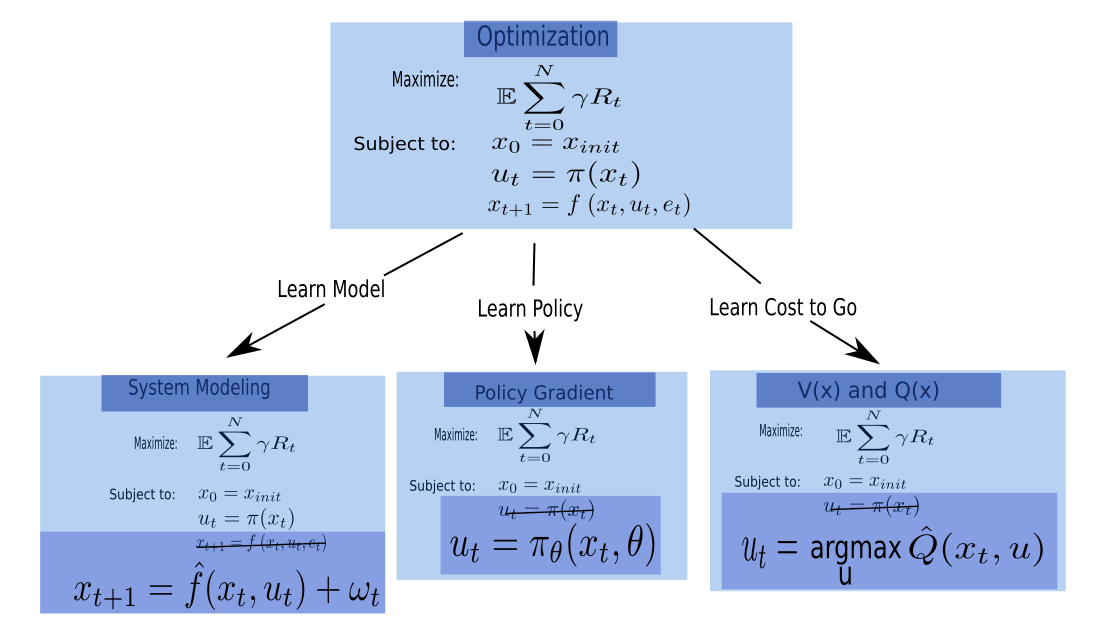
\includegraphics[width=0.5\textwidth]{Control.png}
    \caption{From Optimization to Learning.}
    \label{fig:rl}
\end{figure} 

Model-Based or Model-Free learning refers to whether or not learning is used to approximate the system dynamics function. If there is an explicit action policy, it is called on-policy learning. Otherwise, the optimal action would be implicitly captured by the Q value function, which would be called off-policy learning instead. Importance sampling allows "limited off-policy learning" capacity, which enables data reuse in a trusted region. Online learning means interleaving data collection and iterative network parameters update. Offline learning means the data is collected in bulk first, and then the network parameters are set with regression computation. Batch learning, as the name suggested, is in between online and offline learning. An agent would first generate data that fill its batch memory and then sample from the batch memories for iterative parameter update. Generate new data with the updated parameters. This taxonomy is somewhat outdated now. When Richard Sutton wrote his book\cite{Sutton1998IntroductionTR}, the algorisms he had in mind fall nicely into various categories. Today, however, the popular algorisms would combine more than one route to derive superior performance and can't be pigeonholed.

A fundamental concept for RL is convergence through bootstrap. Instead of asymptotically approaching a known target function, the bootstrap method converges to an assumed target first and then update the target assumption based on collected data. When evaluating estimation functions with belief rather than the real value, things could just run around in circles and never converge. Without any guidance, the RL agent would have explored all the possible states, potentially resulting in this unstable behavior. 

How to collect data in the most efficient manner (Exploration Exploitation Trade-off) and avoid the instability mentioned above in the bootstrap process is a primary focus of researchers. One such method is to give more weight to critical states. Not all observational states are created equal. Some are vital, while others have nothing to do with the eventual objective. For instance, in the inverted pendulum task, any states outside of the Lyapunov stability bounds should be ignored since they would lead to an episode's eventual termination anyway.  

There are statistical techniques to distinguish critical states from the non-essential ones, and imitation learning works by marking crucial states with demonstrations. However, the former approach is hard to implement, and the latter one requires high-quality controllers. Our proposed controller-based coaching method is easy to implement and does not have stringent requirements on the controllers it uses.


Controller-based coaching works by adjusting the RL agent's trajectory and avoid wasting valuable data collection cycle on the states that merely lead to eventual termination. When the agent is about to deviate from essential states, the controller will apply a force to nudge the agent back to where it should be, much like a human coach course-corrects on behalf of the athlete. 

Crucially, the agent is oblivious to this intervention step, and it would not be part of the agent's data. Even if the controller didn't adjust the agent to where it should be, it would not have mattered since the RL agent is headed towards an episode's termination. 

On the other hand, if the controller successfully adjusts the trajectory, the RL agent's next data collection cycle will be spent in a critical state. Therefore, all we require of the PID controller is a reasonable success rate in adjusting the RL agent's trajectory. We test our approach on four mujoco locomotion environments as a proof of concept, and in all four experiments, the hypothesized acceleration on RL training is observed.

\section{Experiment Setup}
Mujoco physics engine\cite{6386109}, is one of many such simulation tools. We interface with it through a python wrapper provided by the OpenAI Gym\cite{Brockman2016OpenAIG}. We choose two environments for our experiments as a proof of concept: inverted pendulum, double inverted pendulum. 

Every environment comes with a set of predetermined rewards and maximum episode steps. We did not tinker with those parameters. The only change we made to each environment is a controller-based coach ready to intervene when the agent steps out of the predetermined critical states.

We use tensorforce's\cite{tensorforce} implementation of RL agents, specifically the Proximal Policy Optimization (PPO) agent because the learning curves generated by PPO agent are smoother, as shown by the spinning up\cite{SpinningUp2018} team. Our paper aims to indicate the controller-based coaching method's feasibility, and a smoother curve makes things easier. 

In this paper, human judgment is the basis for the determination of critical states. In future works, we would like to provide a more systematic process for critical states' demarkation. We will provide our reasonings when we discuss our experiments in each environment. 

Our experiments' code and data can be accessed via \href{https://github.com/BaiLiping/Coaching}{this deposite}. The folders are named after each environment, and in each folder, you will find a data record, an RL agent record, a agent.json file that indicates all the hyperparameters of the RL agent, a Normal file that trains an RL agent with the normal method, a Coached file which trains an agent based on the controller based coaching method, a PID file which is the PID coach. In the PIDvsRL folder, you will find files that generate all the plots shown in the following section.
\subsection{Inveretd Pendulum}
The observation space of the inverted pendulum environment is: [Cart Position on X-axis, Cart Velocity, Pole Angle, Pole Angular Velocity]. The continuous action space is an action ranging from -1 to 1, where -1 means the actuator moves the cart to the left with maximum power and 1 means the actuator moves the cart to the right with full force. The maximum episode step number is 1000. The terminal state for the inverted pendulum is an angle of absolute value greater than 0.2 radius. The reward is 1 for each non-terminal step and 0 for the terminal step. 

Figure\ref{fig:ip} shows how the PID controller manages the pole angle and its angular velocity. The PID parameters are the following: kp=30,ki=0.01,kd=2.26. While the PID controller tries hard to converge to zero, eventually, there would be too much accumulation on the x-axis, and the equilibrium breaks down. The average score achieved by the PID controller is 240.


\begin{figure}[H]
\centering
\begin{subfigure}{0.25\textwidth}
  \centering
  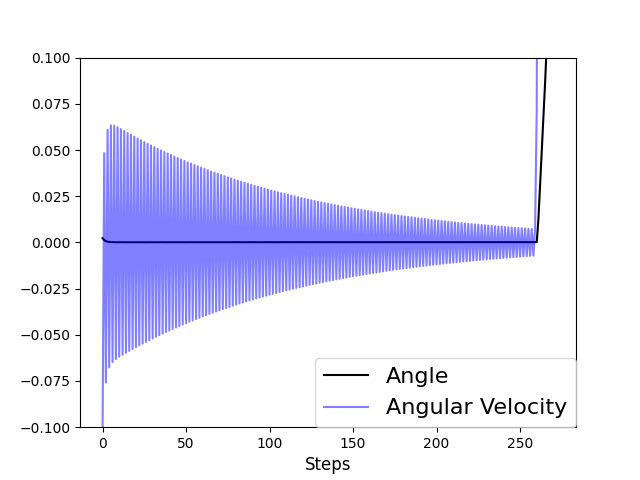
\includegraphics[width=\linewidth]{ip_PID.png}
  \label{fig:ip_pid}
\end{subfigure}%
\begin{subfigure}{.25\textwidth}
  \centering
  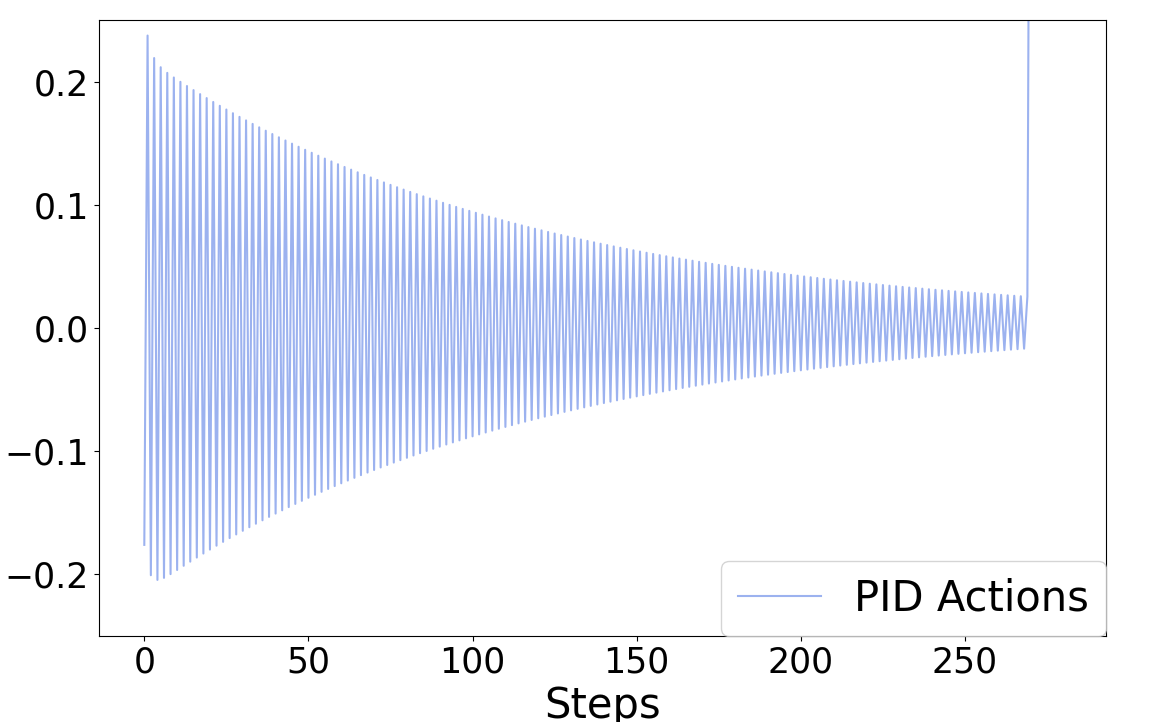
\includegraphics[width=\linewidth]{ip_PID_actions.png}
  \label{fig:ip_pid_actions}
\end{subfigure}
\caption{Inverted Pendulum system controlled by the PID coach. The left plot is the angle and angular velocity against steps, and the right plot is the action against steps. The maximum episode steps are 1000 and each step without termination is scored 1 point. The average score achieved by the PID controller is 240 out of 1000.}
\label{fig:ip}
\end{figure}

Based on our observations of the system, we decide to put the boundary between critical and noncritical states on the angular velocity with an absolute value of 0.4. The RL agent is free to explore with the angular velocity with an absolute value smaller than 0.4, but once it goes above this bound, the PID controller will kick in, trying to decrease the velocity back to the 0.4 bound.
\begin{figure}[H]
     \centering
      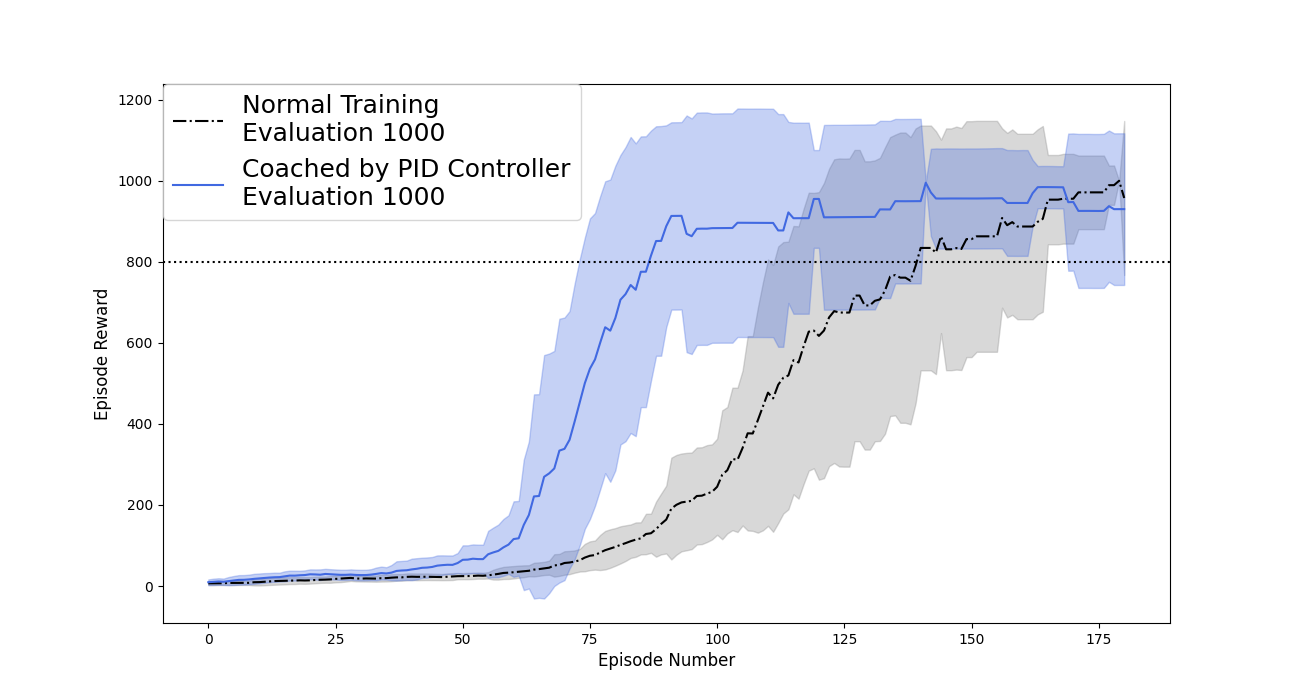
\includegraphics[width=0.5\textwidth]{ip.png}
      \caption{Inverted Pendulum Experiment Result. The lines are the average over 20 episodes, and the shadow indicates the standard deviation over the 20 episodes. The blue line is the training result of RL agent with PID as a coach. The black line is the benchmark of RL agent trained without PID as a coach. }
      \label{fig:ip_result}

\end{figure}

The experiment result is presented by Figure\ref{fig:ip_result}. The black line indicates the agent trained normally, and the blue line indicates the agent trained with a PID coach. A win is set to be with a score greater than 800. It takes the normal method 160 episodes to get five consecutive wins, and it takes the controller-based coaching method 90 episodes to do the same, a 43.8\% increase is observed. As measured by averaging over 20 episodes, it takes the normal method 159 episodes to go beyond 800, and it takes the controller-based coaching method 91 episodes to do the same. A 42.8\% increase is observed. On average, the acceleration brought about by a PID controller, which can only score 240 out of 1000 is 43.3\%\. The agents trained with both methods pass the evaluation, and their respective average scores are presented in the upper left corner. The final performance of the RL agent is shown by Figure\ref{fig:ip_rl}.

\begin{figure}[H]
\centering
\begin{subfigure}{0.25\textwidth}
  \centering
  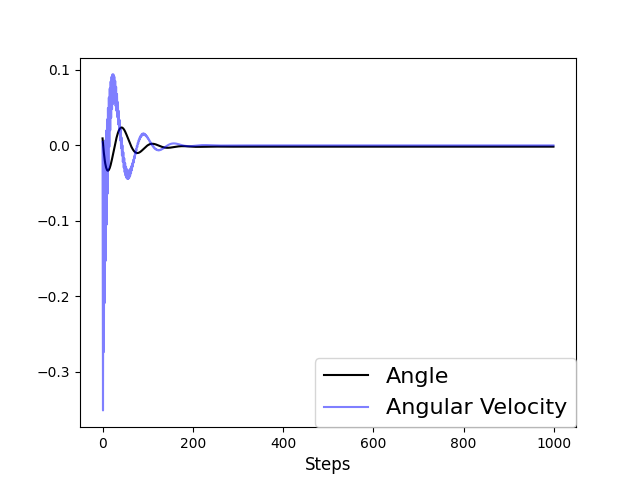
\includegraphics[width=\linewidth]{ip_RL.png}
  \label{fig:ip_pid}
\end{subfigure}%
\begin{subfigure}{.25\textwidth}
  \centering
  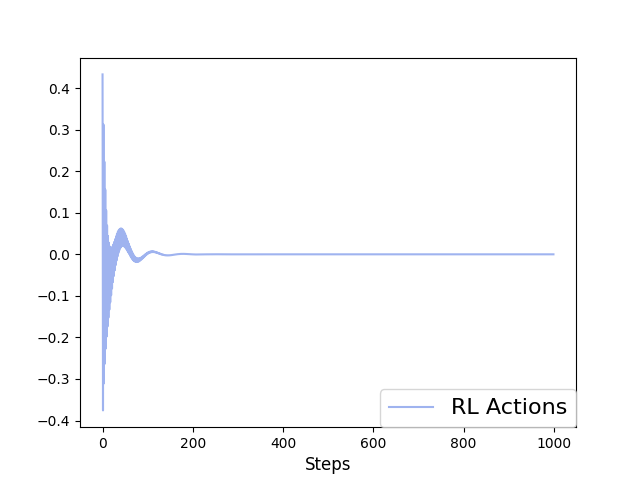
\includegraphics[width=\linewidth]{ip_RL_actions.png}
  \label{fig:ip_pid_actions}
\end{subfigure}
\caption{Inverted Pendulum system controlled by the RL agent. The left plot is the angle and angular velocity against steps, and the right plot is the action against steps. The average score achieved by the RL agent is 1000 out of 1000.}
\label{fig:ip_rl}
\end{figure}

\subsection{Inverted Double Pendulum}
The inverted double pendulum has observation space of the following: [x position of the cart, sin($\theta_1$), sin($\theta_2$),cos($\theta_1$),cos($\theta_2$),velocity of x, angular velocity of $\theta_1$, angular velocity of $\theta_2$, constraint force on x, constraint force on $\theta_1$, constraint force on $\theta_2$]. $\theta_1$ and $\theta_2$ are the angles of the upper and lower pole perspectively. The action space for Inverted Double Pendulum is an action ranging from -10 to 10, where -10 means the actuator moves the cart to the left with maximum power and 10 means the actuator moves the cart to the right with maximum power. A score of roughly 10 points is assigned to non-terminal states, based on the velocity on the x-axis. The detailed formula for score computation can be found at the OpenAI site.

Figure\ref{fig:double} shows how the PID controller manages the lower pole angle and its angular velocity. The parameters of the PID coach is the following: kp=[-0.5,-0.5], ki=[-0.04,-0.003], kd=[-2.95,-0.56]. The actuator action is computed with the following formula: action=kp[0]*lower angle+ki[0]*integral of lower angle+kd[0]*angular velocity of lower angle+kp[1]*upper angle+ki[1]*integral of upper angle+kd[1]*angular velocity of upper angle. The PID controller functions well until the equilibrium breaks down with too much disposition on the x-axis. The average score achieved by the RL agent is 9319, and the average score achieved by the PID controller is 1107.

\begin{figure}[H]
\centering
\begin{subfigure}{0.25\textwidth}
  \centering
  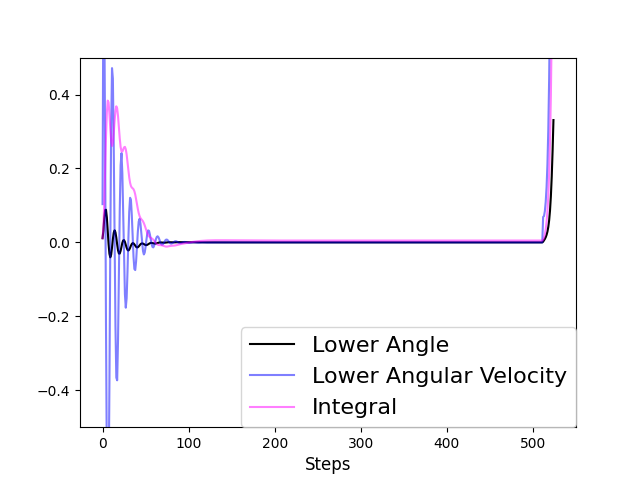
\includegraphics[width=\linewidth]{double_PID.png}
\end{subfigure}%
\begin{subfigure}{.25\textwidth}
  \centering
  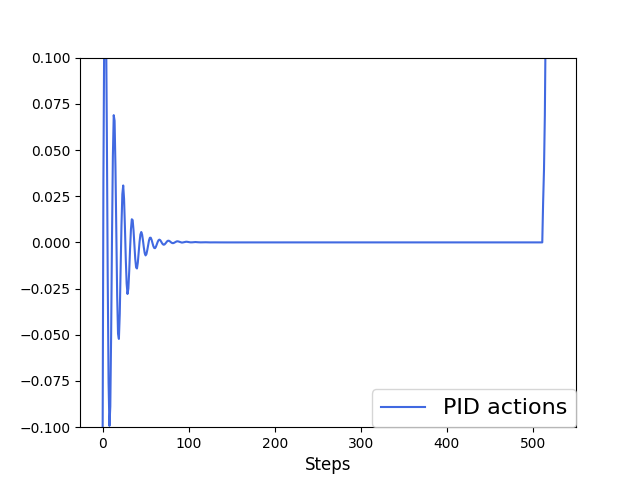
\includegraphics[width=\linewidth]{double_PID_actions.png}
\end{subfigure}
\caption{Inverted Double Pendulum system controlled the PID coach. The left plot is the angle and angular velocity against steps, and the right plot is the action against steps. The maximum episode steps are 1000 and each step without termination is scored at around 10 points, based on velocity on the x axis. The average score achieved by the PID controller is 1107 out of 10000. }
\label{fig:double}
\end{figure}

Based on our observation of the system, we decided to put the boundary between critical and noncritical states on the lower angle of with an absolute value of 0.2. The RL agent is free to explore with the lower angle with an absolute value smaller than 0.2, but once it goes above this bound, the PID controller will kick in, trying to nudge the lower angle back to the 0.2 bound.

\begin{figure}[H]
     \centering
      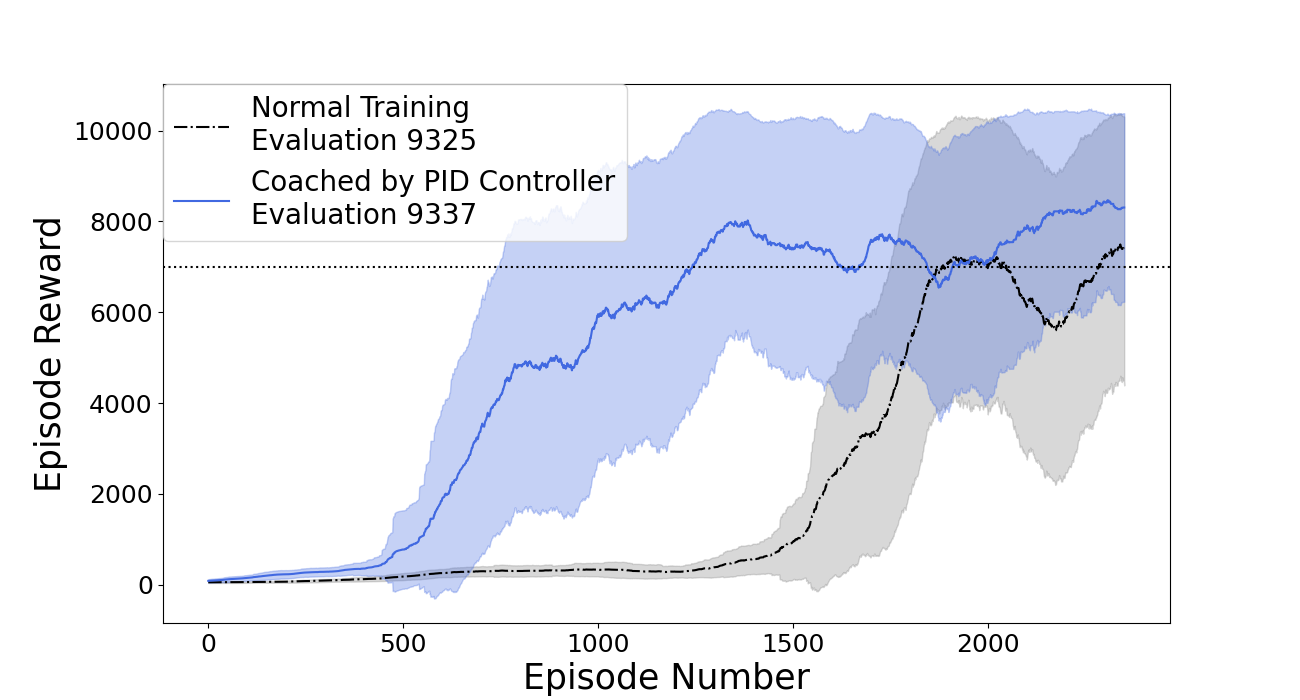
\includegraphics[width=0.5\textwidth]{double.png}
      \caption{Double Inverted Pendulum Coaching Result.}
      \label{fig:double_result}
\end{figure}

The experiment result is presented by Figure\ref{fig:double_result}. The black line indicates the agent trained normally, and the blue line indicates the agent trained with a PID coach. A win is set to be with a score greater than 7000. It takes the normal method 1909 episodes to get five consecutive wins, and it takes controller-based coaching method 1024 episodes to do the same. An increase of 46.3\% is observed. As measured by averaging over 100 episodes, it takes normal method 2031 episodes to go beyond 7000, and it takes controller-based coaching method 1391 episodes to do the same. An increase of 31.5\% is observed. The discrepancy between the two measurements is that the agent trained with the PID controller has a higher variance in its performance. On average, the acceleration brought about by the PID controller is 38.9\%. The agents trained with both methods pass the evaluation, and their respective average scores are presented in the upper left corner. The final performance of the RL agent is shown by Figure\ref{fig:double_rl}.

\begin{figure}[H]
\centering
\begin{subfigure}{0.25\textwidth}
  \centering
  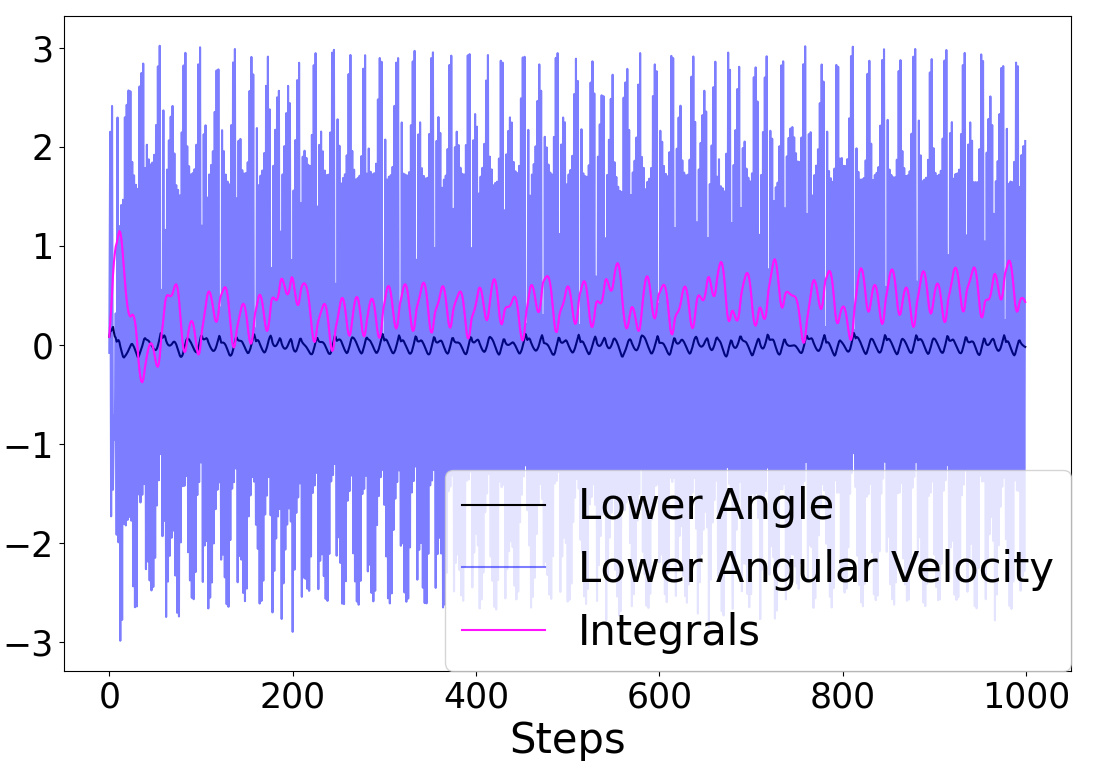
\includegraphics[width=\linewidth]{double_RL.png}
\end{subfigure}%
\begin{subfigure}{.25\textwidth}
  \centering
  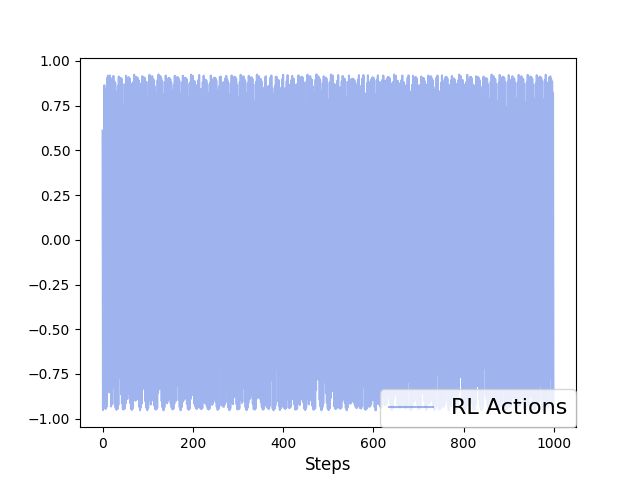
\includegraphics[width=\linewidth]{double_RL_actions.png}
\end{subfigure}
\caption{Inverted Double Pendulum system controlled the RL agent. The left plot is the angle and angular velocity against steps, and the right plot is the action against steps. The average score achieved by the RL agent is 9319 out of 10000.}
\label{fig:double_rl}
\end{figure}


\section{Conclution}

In this paper, we present the controller based coaching approach for accelerated RL training. Unlike previous attempts for using the controller as a guide to RL agent, our method can work with the most primitive PID controllers. In both our experiments, the PID controllers can only score a fraction of the full scores, yet acceleration is still observed. We ascribe this to the fact that the coach intervention step is not part of the RL agent record. Therefore, even if the coach failed to do its job, it would not have worsened the RL training process. Yet when the coach does its job, accelerated data collection on the critical states is achieved. 

Next step, we plan to implement the controller-based coaching idea to the deep drone acrobat project \cite{Kaufmann2020DeepDA}. The drones are trained in simulation, and we think our approach can significantly accelerate their training. In future works, we want to provide a theoretical basis for distinguishing between critical and noncritical states, as opposed to base solely on human judgment, as we did here. 

We believe our research opens the door to a rich reservoir of potential research on coaching RL agents with controllers. Human achieves superhuman feats not because of talent, but because of the meticulously engineered coaching tactics. Current research in RL focuses solely on the "athlete" side of the equation, i.e., building an efficient RL agent, but we feel "coach" is as important, if not more so.  For instance, a tennis coach will challenge athletes, pushing them to experience situations that are hard to encounter. A controller can function as a coach and pushes the RL agent into states that are hard to access. Controller-based coaching can be an effective way to merge controllers with RL agents. 

\bibliographystyle{IEEEtran}
\bibliography{Bibliography}
%\printbibliography

\end{document}